\chapter{Матрицалар}

\index{матрица}

\key{Матрица} бағдарламалаудағы екі өлшемді жиымға сәйкес
математикалық тұжырымдама. Мысалы:

% A \key{matrix} is a mathematical concept
% that corresponds to a two-dimensional array
% in programming. For example,
\[
A = 
 \begin{bmatrix}
  6 & 13 & 7 & 4 \\
  7 & 0 & 8 & 2 \\
  9 & 5 & 4 & 18 \\
 \end{bmatrix}
\]
-- $3 \times 4$ өлшемді матрица, яғни 
3 жолы және 4 бағанасы бар.
$[i,j]$ нотациясы $i$-жолда және
$j$-бағанда тұрған элементке сілтейді.
Мысалы жоғарыдағы матрицада $A[2,3]=8$
және $A[3,1]=9$.

\index{вектор}

Матрицаның ерекше жағдайы -- \key{вектор}. Ол --
өлшемі $n \times 1$ болатын матрица. 
Мысалы: 
% A special case of a matrix is a \key{vector}
% that is a one-dimensional matrix of size $n \times 1$.
\[
V =
\begin{bmatrix}
4 \\
7 \\
5 \\
\end{bmatrix}
\]
-- үш элементті қамтитын вектор. 

\index{аудару}

$A$ матрицаның \key{аударуы} $A^T$–ны
$A$ матрицасының 
жолдарымен бағаналарын ауыстыру арқылы алынады,
яғни $A^T[i,j]=A[j,i]$:
% The \key{transpose} $A^T$ of a matrix $A$
% is obtained when the rows and columns of $A$
% are swapped, i.e., $A^T[i,j]=A[j,i]$:
\[
A^T = 
 \begin{bmatrix}
  6 & 7 & 9 \\
  13 & 0 & 5 \\
  7 & 8 & 4 \\
  4 & 2 & 18 \\
 \end{bmatrix}
\]

\index{шаршы матрица}

Егер
жолдар саны мен бағана саны бірдей болса, ондай матрица \key{шаршы матрица} деп аталады. 
Мысалы төменде шаршы матрица берілген:
\[
S = 
 \begin{bmatrix}
  3 & 12 & 4  \\
  5 & 9 & 15  \\
  0 & 2 & 4 \\
 \end{bmatrix}
\]

\section{Операциялар}

$A$ мен $B$ матрицаларының қосындысы 
$A+B$ анықталған. Егер матрицалардың 
өлшемдері бірдей болса, нәтижесінде әр элементі сәйкес $A$ және $B$ элементтерінің қосындысын беретін матрица пайда болады.

% TODO
% The result is a matrix where each element
% is the sum of the corresponding elements
% in $A$ and $B$.

Мысалы
\[
 \begin{bmatrix}
  6 & 1 & 4 \\
  3 & 9 & 2 \\
 \end{bmatrix}
+
 \begin{bmatrix}
  4 & 9 & 3 \\
  8 & 1 & 3 \\
 \end{bmatrix}
=
 \begin{bmatrix}
  6+4 & 1+9 & 4+3 \\
  3+8 & 9+1 & 2+3 \\
 \end{bmatrix}
=
 \begin{bmatrix}
  10 & 10 & 7 \\
  11 & 10 & 5 \\
 \end{bmatrix}.
\]

$A$ матрицасын $x$ мәніне көбейту деген сөз
$A$ әр элементінің $x$-ке көбейтілетінін 
білдіреді.

Мысалы
\[
 2 \cdot \begin{bmatrix}
  6 & 1 & 4 \\
  3 & 9 & 2 \\
 \end{bmatrix}
=
 \begin{bmatrix}
  2 \cdot 6 & 2\cdot1 & 2\cdot4 \\
  2\cdot3 & 2\cdot9 & 2\cdot2 \\
 \end{bmatrix}
=
 \begin{bmatrix}
  12 & 2 & 8 \\
  6 & 18 & 4 \\
 \end{bmatrix}.
\]

\subsubsection{Матрицаларды көбейту}

\index{матрицаларды көбейту}

Егер $A$-ның өлшемі 
$a \times n$ және $B$-ның өлшемі 
$n \times b$ (яғни $A$-ның ені $B$-ның
биіктігіне тең) болса, $A$ мен $B$ матрицаларының көбейтіндісі 
$AB$ анықталған болады. Төменде көбейтіндісі 
\[
AB[i,j] = \sum_{k=1}^n A[i,k] \cdot B[k,j].
\]
формуласы арқылы есептелген $a \times b$ өлшемді
матрица беріледі. 

Яғни $AB$-ның әр элементі төмендегі суреттегідей
$A$ мен $B$ элементтері көбейтінділерінің қосындысына тең болады:

\begin{center}
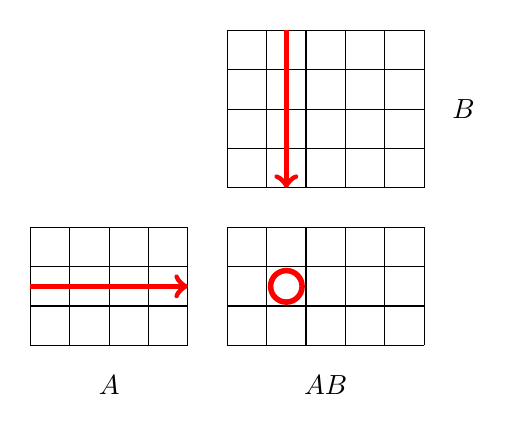
\begin{tikzpicture}[scale=0.5]
\draw (0,0) grid (4,3);
\draw (5,0) grid (10,3);
\draw (5,4) grid (10,8);

\node at (2,-1) {$A$};
\node at (7.5,-1) {$AB$};
\node at (11,6) {$B$};

\draw[thick,->,red,line width=2pt] (0,1.5) -- (4,1.5);
\draw[thick,->,red,line width=2pt] (6.5,8) -- (6.5,4);
\draw[thick,red,line width=2pt] (6.5,1.5) circle (0.4);
\end{tikzpicture}
\end{center}

Мысалы:

\[
 \begin{bmatrix}
  1 & 4 \\
  3 & 9 \\
  8 & 6 \\
 \end{bmatrix}
\cdot
 \begin{bmatrix}
  1 & 6 \\
  2 & 9 \\
 \end{bmatrix}
=
 \begin{bmatrix}
  1 \cdot 1 + 4 \cdot 2 & 1 \cdot 6 + 4 \cdot 9 \\
  3 \cdot 1 + 9 \cdot 2 & 3 \cdot 6 + 9 \cdot 9 \\
  8 \cdot 1 + 6 \cdot 2 & 8 \cdot 6 + 6 \cdot 9 \\
 \end{bmatrix}
=
 \begin{bmatrix}
  9 & 42 \\
  21 & 99 \\
  20 & 102 \\
 \end{bmatrix}.
\]

Матрицадағы көбейту –– ассоциативті,
яғни $A(BC)=(AB)C$, бірақ коммутативті 
емес, яғни әдетте $AB = BA$ болмайды.

\index{бірлік матрица}

\key{Бірлік матрица} –– диагоналдағы элементтері бірге 
тең және қалған элементтері нөлге тең шаршы матрица.
Мысалы, төменде $3 \times 3$ өлшемді бірлік матрица келтірілген:
\[
 I = \begin{bmatrix}
  1 & 0 & 0 \\
  0 & 1 & 0 \\
  0 & 0 & 1 \\
 \end{bmatrix}
\]

\begin{samepage}
Бірлік матрицаға көбейтілген матрица өзгермейді.
Мысалы:
\[
 \begin{bmatrix}
  1 & 0 & 0 \\
  0 & 1 & 0 \\
  0 & 0 & 1 \\
 \end{bmatrix}
\cdot
 \begin{bmatrix}
  1 & 4 \\
  3 & 9 \\
  8 & 6 \\
 \end{bmatrix}
=
 \begin{bmatrix}
  1 & 4 \\
  3 & 9 \\
  8 & 6 \\
 \end{bmatrix} \hspace{10px} \textrm{және} \hspace{10px}
 \begin{bmatrix}
  1 & 4 \\
  3 & 9 \\
  8 & 6 \\
 \end{bmatrix}
\cdot
 \begin{bmatrix}
  1 & 0 \\
  0 & 1 \\
 \end{bmatrix}
=
 \begin{bmatrix}
  1 & 4 \\
  3 & 9 \\
  8 & 6 \\
 \end{bmatrix}.
\]
\end{samepage}

Қарапайым алгоритм арқылы екі $n \times n$
матрицаларының көбейтіндісін $O(n^3)$
уақытта есептеуге болады. Матрицалардың
көбейтіндісін есептейтін одан да
тиімді алгоритмдер бар\footnote{Сондай алгоритмдердің
алғашқысын 1969 жылы Штрассен ойлап тапты \cite{str69}.
Қазір алгоритм оның атымен аталады.
Оның уақытша күрделілігі -- $O(n^{2.80735})$;
бүгінге дейін ең тиімді алгоритм
$O(n^{2.37286})$ уақытта жұмыс істейді \cite{gal14}.},
бірақ оларға теориялық тұрғыдан қызығушылық танытқанымызбен, жарыстарда қолдана бермейміз. 

\subsubsection{Матрица дәрежесі}

\index{матрица дәрежесі}

Егер $A$ матрицасы шаршы матрица болса, онда $A$ матрицасының дәрежесі $A^k$ анықталған болады.
 
Оның анықтамасы матрицаларды көбейтуге негізделеді:
\[ A^k = \underbrace{A \cdot A \cdot A \cdots A}_{\textrm{$k$ рет}} \]
Мысалы

\[
 \begin{bmatrix}
  2 & 5 \\
  1 & 4 \\
 \end{bmatrix}^3 =
 \begin{bmatrix}
  2 & 5 \\
  1 & 4 \\
 \end{bmatrix} \cdot
 \begin{bmatrix}
  2 & 5 \\
  1 & 4 \\
 \end{bmatrix} \cdot
 \begin{bmatrix}
  2 & 5 \\
  1 & 4 \\
 \end{bmatrix} =
 \begin{bmatrix}
  48 & 165 \\
  33 & 114 \\
 \end{bmatrix}.
\]
Оған қоса, $A^0$ бірлік матрицаға тең болады. Мысалы
\[
 \begin{bmatrix}
  2 & 5 \\
  1 & 4 \\
 \end{bmatrix}^0 =
 \begin{bmatrix}
  1 & 0 \\
  0 & 1 \\
 \end{bmatrix}.
\]

$A^k$ матрицасын 21.2-тарауда айтылған алгоритм арқылы
$O(n^3 \log k)$ уақыт ішінде
тиімді есептеуімізге болады. Мысалы:
\[
 \begin{bmatrix}
  2 & 5 \\
  1 & 4 \\
 \end{bmatrix}^8 =
 \begin{bmatrix}
  2 & 5 \\
  1 & 4 \\
 \end{bmatrix}^4 \cdot
 \begin{bmatrix}
  2 & 5 \\
  1 & 4 \\
 \end{bmatrix}^4.
\]

\subsubsection{Анықтауыш}

\index{анықтауыш}

Егер $A$ шаршы матрица болса, $A$ матрицасының \key{анықтауышы} $\det(A)$
анықталған болады. 
$A$-ның өлшемі $1 \times 1$ болса,
онда $\det(A)=A[1,1]$. Одан үлкен матрицаның
анықтауышы рекурсивті формула 
арқылы есептелінеді. \index{алгебралық толықтауыш}
\[\det(A)=\sum_{j=1}^n A[1,j] C[1,j],\]
мұндағы $C[i,j]$ -- $[i,j]$ позициясының \key{алгебралық толықтауышы}.
Алгебралық толықтауыш төмендегі формула арқылы есептелінеді:
\[C[i,j] = (-1)^{i+j} \det(M[i,j]),\]
мұндағы $M[i,j]$ ––
$i$-жолы мен $j$-бағанасы өшірілген $A$ матрицасы.
Алгебралық толықтауыштың $(-1)^{i+j}$ коэффициентіне байланысты
анықтауыштар аралата келе, оң және теріс болып бөлінеді. 
Мысалы
\[
\det(
 \begin{bmatrix}
  3 & 4 \\
  1 & 6 \\
 \end{bmatrix}
) = 3 \cdot 6 - 4 \cdot 1 = 14 
\]
және
\[
\det(
 \begin{bmatrix}
  2 & 4 & 3 \\
  5 & 1 & 6 \\
  7 & 2 & 4 \\
 \end{bmatrix}
) = 
2 \cdot
\det(
 \begin{bmatrix}
  1 & 6 \\
  2 & 4 \\
 \end{bmatrix}
)
-4 \cdot
\det(
 \begin{bmatrix}
  5 & 6 \\
  7 & 4 \\
 \end{bmatrix}
)
+3 \cdot
\det(
 \begin{bmatrix}
  5 & 1 \\
  7 & 2 \\
 \end{bmatrix}
) = 81.
\]

\index{кері матрица}

$A$–ның анықтауышы матрицаның \key{кері 
матрицасы} $A^{-1}$ бар-жоғын айтады.
Кері матрица дегеніміз $A \cdot A^{-1} = I$
орындалатын $A^{-1}$ матрицасы, мұндағы 
$I$ бірлік матрицасы. Егер
$\det(A) \neq 0$ болса ғана, $A^{-1}$ кері матрицасы бар болады және оны төмендегі формула
бойынша есептей аламыз:

\[A^{-1}[i,j] = \frac{C[j,i]}{det(A)}.\]

Мысалы:

\[
\underbrace{
 \begin{bmatrix}
  2 & 4 & 3\\
  5 & 1 & 6\\
  7 & 2 & 4\\
 \end{bmatrix}
}_{A}
\cdot
\underbrace{
 \frac{1}{81}
 \begin{bmatrix}
   -8 & -10 & 21 \\
   22 & -13 & 3 \\
   3 & 24 & -18 \\
 \end{bmatrix}
}_{A^{-1}}
=
\underbrace{
 \begin{bmatrix}
  1 & 0 & 0 \\
  0 & 1 & 0 \\
  0 & 0 & 1 \\
 \end{bmatrix}
}_{I}.
\]

\section{Сызықтық рекуренттілік}

\index{сызықтық рекуренттілік}

\key{Сызықтық рекуренттілік} -- 
бастапқы мәндері 
$f(0),f(1),\ldots,f(k-1)$ болатын
және одан үлкен мәндері 
\[f(n) = c_1 f(n-1) + c_2 f(n-2) + \ldots + c_k f (n-k),\]
рекурсивті формула 
арқылы есептелетін функция, мұндағы $c_1,c_2,\ldots,c_k$ тұрақты
коэффициенттер.

% A \key{linear recurrence}
% is a function $f(n)$
% whose initial values are
% $f(0),f(1),\ldots,f(k-1)$
% and larger values
% are calculated recursively using the formula
% \[f(n) = c_1 f(n-1) + c_2 f(n-2) + \ldots + c_k f (n-k),\]
% where $c_1,c_2,\ldots,c_k$ are constant coefficients.
% TODO CHECK IT THROUGHLY

Динамикалық бағдарламалау арқылы $f(n)$-нің кез келген 
мәнін $O(kn)$ уақытта 
$f(0),f(1),\ldots,f(n)$ мәндерін біртіндеп есептеу арқылы
табуға болады. Бірақ $k$ кішкентай болса, $f(n)$-ді
матрица операциялары арқылы $O(k^3 \log n)$ 
уақытта әлдеқайда тиімдірек есептей аламыз. 

\subsubsection{Фибоначчи сандары}

\index{Фибоначчи сандары}

Сызықтық рекуренттілікке ең қарапайым үлгі 
Фибоначчи сандарын анықтайтын функция болмақ:
\[
\begin{array}{lcl}
f(0) & = & 0 \\
f(1) & = & 1 \\
f(n) & = & f(n-1)+f(n-2) \\
\end{array}
\]
Бұл жағдайда $k=2$ және $c_1=c_2=1$.

\begin{samepage}
Фибоначчи сандарын тиімді есептеу үшін
Фибоначчи формуласын өлшемі $2 \times 2$ 
болатын 
және келесі ара қатынас орындалатын
шаршы матрица $X$ арқылы көрсетейік:
% To efficiently calculate Fibonacci numbers,
% we represent the
% Fibonacci formula as a
% square matrix $X$ of size $2 \times 2$,
% for which the following holds:
\[ X \cdot
 \begin{bmatrix}
  f(i) \\
  f(i+1) \\
 \end{bmatrix}
=
 \begin{bmatrix}
  f(i+1) \\
  f(i+2) \\
 \end{bmatrix}
 \]
Осылайша $f(i)$ және $f(i+1)$ мәндері 
$X$-ке ''енгізу'' ретінде берілген және
$X$ солар арқылы $f(i+1)$ және $f(i+2)$ мәндерін
есептеп береді. $X$ матрицасының мәні төмендегідей болады:

\[ X = 
 \begin{bmatrix}
  0 & 1 \\
  1 & 1 \\
 \end{bmatrix}.
\]
\end{samepage}
\noindent
Мысалы:
\[
 \begin{bmatrix}
  0 & 1 \\
  1 & 1 \\
 \end{bmatrix}
\cdot
 \begin{bmatrix}
  f(5) \\
  f(6) \\
 \end{bmatrix}
=
 \begin{bmatrix}
  0 & 1 \\
  1 & 1 \\
 \end{bmatrix}
\cdot
 \begin{bmatrix}
  5 \\
  8 \\
 \end{bmatrix}
=
 \begin{bmatrix}
  8 \\
  13 \\
 \end{bmatrix}
=
 \begin{bmatrix}
  f(6) \\
  f(7) \\
 \end{bmatrix}.
\]
Осылайша $f(n)$-ді келесі формула арқылы есептеуімізге болады:
\[
 \begin{bmatrix}
  f(n) \\
  f(n+1) \\
 \end{bmatrix}
=
X^n \cdot
 \begin{bmatrix}
  f(0) \\
  f(1) \\
 \end{bmatrix}
=
 \begin{bmatrix}
  0 & 1 \\
  1 & 1 \\
 \end{bmatrix}^n
\cdot
 \begin{bmatrix}
  0 \\
  1 \\
 \end{bmatrix}.
\]
$X^n$ мәні $O(\log n)$ уақытта есептелінеді,
демек $f(n)$-нің мәні де $O(\log n)$ уақытта 
есептелінеді. 

\subsubsection{Жалпы жағдай}

Жалпы сызықтық рекуренттілік $f(n)$ функциясын
қарастырайық. Біздің мақсатымыз қайтадан төмендегі орындалатын
$X$ матрицасын құру

\[ X \cdot
 \begin{bmatrix}
  f(i) \\
  f(i+1) \\
  \vdots \\
  f(i+k-1) \\
 \end{bmatrix}
=
 \begin{bmatrix}
  f(i+1) \\
  f(i+2) \\
  \vdots \\
  f(i+k) \\
 \end{bmatrix}.
\]
Ондай матрицаның түрі осындай болады
\[
X =
 \begin{bmatrix}
  0 & 1 & 0 & 0 & \cdots & 0 \\
  0 & 0 & 1 & 0 & \cdots & 0 \\
  0 & 0 & 0 & 1 & \cdots & 0 \\
  \vdots & \vdots & \vdots & \vdots & \ddots & \vdots \\
  0 & 0 & 0 & 0 & \cdots & 1 \\
  c_k & c_{k-1} & c_{k-2} & c_{k-3} & \cdots & c_1 \\
 \end{bmatrix}.
\]
Бастапқы $k-1$ жолда бір элемент бірге тең және қалған 
элементтер нөлге тең болады. Бұл жолдар 
$f(i)$-ді $f(i+1)$-мен, $f(i+1)$-ді $f(i+2)$-мен,
т.с.с. ауыстырады. Соңғы жол болса, жаңа $f(i+k)$ мәнін 
есептеу үшін рекуренттіліктің коэффициенттерін қамтиды.

\begin{samepage}
Енді $f(n)$ мәнін $O(k^3 \log n)$ уақытта 
төмендегі формула арқылы есептеуімізге болады:
\[
 \begin{bmatrix}
  f(n) \\
  f(n+1) \\
  \vdots \\
  f(n+k-1) \\
 \end{bmatrix}
=
X^n \cdot
 \begin{bmatrix}
  f(0) \\
  f(1) \\
  \vdots \\
  f(k-1) \\
 \end{bmatrix}.
\]
\end{samepage}

\section{Графтар мен матрицалар}

\subsubsection{Жолдар санау}

Графтың cыбайластық матрицасының дәрежесі
қызық қасиетке ие болады. Егер $V$ 
салмақталмаған графтың cыбайластық матрицасы болса,
$V^n$ матрицасы $n$ қыр арқылы өтетін төбелер арасындағы
жолдар санын қамтиды. 

Келесідегі графқа
\begin{center}
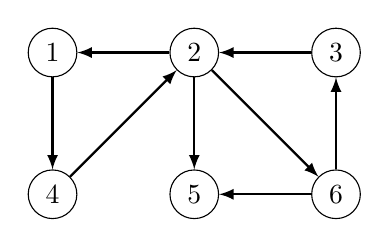
\begin{tikzpicture}[scale=0.9]
\node[draw, circle] (1) at (1,3) {$1$};
\node[draw, circle] (2) at (1,1) {$4$};
\node[draw, circle] (3) at (3,3) {$2$};
\node[draw, circle] (4) at (5,3) {$3$};
\node[draw, circle] (5) at (3,1) {$5$};
\node[draw, circle] (6) at (5,1) {$6$};

\path[draw,thick,->,>=latex] (1) -- (2);
\path[draw,thick,->,>=latex] (2) -- (3);
\path[draw,thick,->,>=latex] (3) -- (1);
\path[draw,thick,->,>=latex] (4) -- (3);
\path[draw,thick,->,>=latex] (3) -- (5);
\path[draw,thick,->,>=latex] (3) -- (6);
\path[draw,thick,->,>=latex] (6) -- (4);
\path[draw,thick,->,>=latex] (6) -- (5);
\end{tikzpicture}
\end{center}
cыбайластық матрица 
\[
V= \begin{bmatrix}
  0 & 0 & 0 & 1 & 0 & 0 \\
  1 & 0 & 0 & 0 & 1 & 1 \\
  0 & 1 & 0 & 0 & 0 & 0 \\
  0 & 1 & 0 & 0 & 0 & 0 \\
  0 & 0 & 0 & 0 & 0 & 0 \\
  0 & 0 & 1 & 0 & 1 & 0 \\
 \end{bmatrix}.
\]
болады. Төмендегі матрица
\[
V^4= \begin{bmatrix}
  0 & 0 & 1 & 1 & 1 & 0 \\
  2 & 0 & 0 & 0 & 2 & 2 \\
  0 & 2 & 0 & 0 & 0 & 0 \\
  0 & 2 & 0 & 0 & 0 & 0 \\
  0 & 0 & 0 & 0 & 0 & 0 \\
  0 & 0 & 1 & 1 & 1 & 0 \\
 \end{bmatrix}
\]
4 төбе арқылы өтетін төбелер арасындағы
жолдар санын қамтиды.
Мысалы, $V^4[2,5]=2$,
себебі 2-төбе мен 5-төбе арасында 
4 қырдан өтетін 2 жол бар:
$2 \rightarrow 1 \rightarrow 4 \rightarrow 2 \rightarrow 5$
және 
$2 \rightarrow 6 \rightarrow 3 \rightarrow 2 \rightarrow 5$.

\subsubsection{Ең қысқа жол}

Дәл жаңағы идеяны салмақталған графта қолдансақ,
$n$ қыр арқылы өтетін төбелер арасындағы минималды жолдың ұзындығын 
есептей аламыз.
Оны есептеу үшін матрицалардың көбейтуін  жолдардың санын санамайтын, бірақ 
жолдардың ұзындығын минималдайтындай жаңа түрде 
анықтауымыз қажет.

\begin{samepage}
Өрнек ретінде төмендегі графты қарастырайық:
\begin{center}
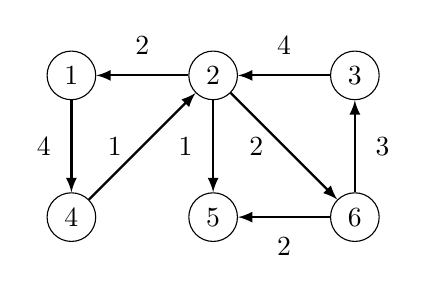
\begin{tikzpicture}[scale=0.9]
\node[draw, circle] (1) at (1,3) {$1$};
\node[draw, circle] (2) at (1,1) {$4$};
\node[draw, circle] (3) at (3,3) {$2$};
\node[draw, circle] (4) at (5,3) {$3$};
\node[draw, circle] (5) at (3,1) {$5$};
\node[draw, circle] (6) at (5,1) {$6$};

\path[draw,thick,->,>=latex] (1) -- node[font=\small,label=left:4] {} (2);
\path[draw,thick,->,>=latex] (2) -- node[font=\small,label=left:1] {} (3);
\path[draw,thick,->,>=latex] (3) -- node[font=\small,label=north:2] {} (1);
\path[draw,thick,->,>=latex] (4) -- node[font=\small,label=north:4] {} (3);
\path[draw,thick,->,>=latex] (3) -- node[font=\small,label=left:1] {} (5);
\path[draw,thick,->,>=latex] (3) -- node[font=\small,label=left:2] {} (6);
\path[draw,thick,->,>=latex] (6) -- node[font=\small,label=right:3] {} (4);
\path[draw,thick,->,>=latex] (6) -- node[font=\small,label=below:2] {} (5);
\end{tikzpicture}
\end{center}
\end{samepage}

Сыбайластық матрицасын құрастырайық. Егер 
қыр болмаса, $\infty$ деп анықтайық, әйтпесе
соған сәйкес мәнімен анықтайық.
Матрица --
\[
V= \begin{bmatrix}
  \infty & \infty & \infty & 4 & \infty & \infty \\
  2 & \infty & \infty & \infty & 1 & 2 \\
  \infty & 4 & \infty & \infty & \infty & \infty \\
  \infty & 1 & \infty & \infty & \infty & \infty \\
  \infty & \infty & \infty & \infty & \infty & \infty \\
  \infty & \infty & 3 & \infty & 2 & \infty \\
 \end{bmatrix}.
\]

Матрицаларды көбейту үшін 
төмендегі формуланың орнына
\[
AB[i,j] = \sum_{k=1}^n A[i,k] \cdot B[k,j]
\]
осы формуланы қолданамыз:
\[
AB[i,j] = \min_{k=1}^n A[i,k] + B[k,j],
\]
демек біз қосындының орнына минимумды және
элементтердің көбейтіндісінің орнына қосындысын
есептейміз.
Осы өзгерістен кейін матрицаның дәрежесі 
графтың ең қысқа жолдарына сәйкес келеді.

Мысалы:
\[
V^4= \begin{bmatrix}
  \infty & \infty & 10 & 11 & 9 & \infty \\
  9 & \infty & \infty & \infty & 8 & 9 \\
  \infty & 11 & \infty & \infty & \infty & \infty \\
  \infty & 8 & \infty & \infty & \infty & \infty \\
  \infty & \infty & \infty & \infty & \infty & \infty \\
  \infty & \infty & 12 & 13 & 11 & \infty \\
 \end{bmatrix},
\]
болғандықтан, 2-төбеден 5-төбеге дейін 4 қыр арқылы 
өтетін жолдың ең қысқа ұзындығы 8 болатынын қорытындылай аламыз.
Ол жол --
$2 \rightarrow 1 \rightarrow 4 \rightarrow 2 \rightarrow 5$.

\subsubsection{Кирхгоф теоремасы}

\index{Кирхгоф теоремасы}
\index{қаңқалы дарақ}

\key{Кирхгоф теоремасы}
%\footnote{G. R. Kirchhoff (1824--1887) was a German physicist.}
арнайы матрицаның анықтауышы арқылы
графтың қаңқалы дарақтарының санын табуға
мүмкіндік береді.
Мысалы, төмендегі графта
\begin{center}
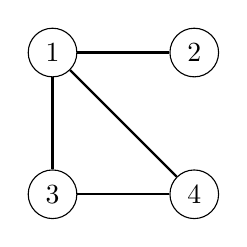
\begin{tikzpicture}[scale=0.9]
\node[draw, circle] (1) at (1,3) {$1$};
\node[draw, circle] (2) at (3,3) {$2$};
\node[draw, circle] (3) at (1,1) {$3$};
\node[draw, circle] (4) at (3,1) {$4$};

\path[draw,thick,-] (1) -- (2);
\path[draw,thick,-] (1) -- (3);
\path[draw,thick,-] (3) -- (4);
\path[draw,thick,-] (1) -- (4);
\end{tikzpicture}
\end{center}
үш қаңқалы дарақ бар:
\begin{center}
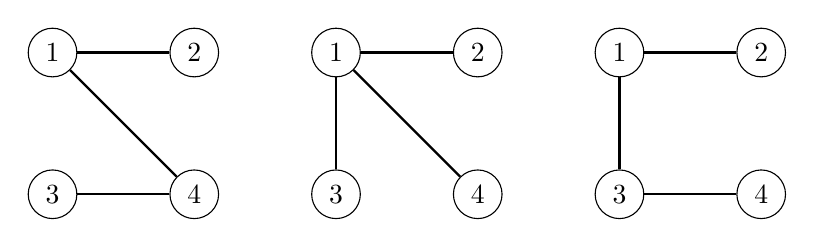
\begin{tikzpicture}[scale=0.9]
\node[draw, circle] (1a) at (1,3) {$1$};
\node[draw, circle] (2a) at (3,3) {$2$};
\node[draw, circle] (3a) at (1,1) {$3$};
\node[draw, circle] (4a) at (3,1) {$4$};

\path[draw,thick,-] (1a) -- (2a);
%\path[draw,thick,-] (1a) -- (3a);
\path[draw,thick,-] (3a) -- (4a);
\path[draw,thick,-] (1a) -- (4a);

\node[draw, circle] (1b) at (1+4,3) {$1$};
\node[draw, circle] (2b) at (3+4,3) {$2$};
\node[draw, circle] (3b) at (1+4,1) {$3$};
\node[draw, circle] (4b) at (3+4,1) {$4$};

\path[draw,thick,-] (1b) -- (2b);
\path[draw,thick,-] (1b) -- (3b);
%\path[draw,thick,-] (3b) -- (4b);
\path[draw,thick,-] (1b) -- (4b);

\node[draw, circle] (1c) at (1+8,3) {$1$};
\node[draw, circle] (2c) at (3+8,3) {$2$};
\node[draw, circle] (3c) at (1+8,1) {$3$};
\node[draw, circle] (4c) at (3+8,1) {$4$};

\path[draw,thick,-] (1c) -- (2c);
\path[draw,thick,-] (1c) -- (3c);
\path[draw,thick,-] (3c) -- (4c);
%\path[draw,thick,-] (1c) -- (4c);
\end{tikzpicture}
\end{center}
\index{Лаплас матрицасы}
Қаңқалы дарақтардың санын санау үшін 
\key{Лаплас матрицасын} $L$ құрайық. 
Матрицада $L[i,i]$ $i$-төбенің дәрежесіне тең
және егер $i$ мен $j$ арасында қыр болса,
$L[i,j]=-1$, әйтпесе $L[i,j]=0$ тең.
Жоғарыдағы графқа сәйкес Лаплас матрицасы 
төмендегідей болады
\[
L= \begin{bmatrix}
  3 & -1 & -1 & -1 \\
  -1 & 1 & 0 & 0 \\
  -1 & 0 & 2 & -1 \\
  -1 & 0 & -1 & 2 \\
 \end{bmatrix}
\]

Егер $L$ матрицасының кез келген жолы мен
бағанасын өшіріп, оның анықтауышын қарасақ,
ол қаңқалы дарақтардың санына тең екенін
көреміз. 

Мысалы егер бірінші жол мен біріші бағананы 
өшірсек, нәтижесінде

\[ \det(
\begin{bmatrix}
  1 & 0 & 0 \\
  0 & 2 & -1 \\
  0 & -1 & 2 \\
 \end{bmatrix}
) =3.\]
$L$ матрицасының қандай да болсын жолы мен 
бағанасын өшірсек, анықтауышы әрдайым бірдей 
болады.

22.5-тарауындағы Кэли формуласы 
Кирхгоф теоремасының дербес жағдайы
екенін көруімізге болады,
себебі $n$ төбелі толық граф төмендегідей болмақ: 

\[ \det(
\begin{bmatrix}
  n-1 & -1 & \cdots & -1 \\
  -1 & n-1 & \cdots & -1 \\
  \vdots & \vdots & \ddots & \vdots \\
  -1 & -1 & \cdots & n-1 \\
 \end{bmatrix}
) =n^{n-2}.\]



